\section{CateEA: Enhancing Entity Alignment via Implicit Category Supervision}

\subsection{Ý tưởng chính} %Hùng
% Giải thích ý tưởng cốt lõi bằng ví dụ, không lặp lại định nghĩa MMEA.
Các phương pháp MMEA hiện tại thường tổng hợp các nguồn thông tin của thực thể (cấu trúc, quan hệ, thuộc tính, tên, hình ảnh) thành một vector duy nhất, rồi so sánh độ tương đồng giữa các vector này để chọn ra các thực thể tương ứng. Tuy nhiên, độ đo này không phải lúc nào cũng thể hiện đúng tính tương đương của hai thực thể. Ví dụ ở hình~\ref{fig:cateea_idea}, thực thể "Chow Chow" (một giống chó) và "Lion" (sư tử) có thể bị căn chỉnh nhầm với nhau vì hình ảnh của chúng có nhiều nét giống nhau, trong khi thực tế đây là hai loài khác nhau. Mô hình chỉ nhìn vào độ tương đồng của vector đặc trưng nên không biết được hai thực thể này thuộc hai danh mục khác nhau, trong khi con người nhìn vào là phân biệt được ngay.

\begin{figure}[htp]
\centering
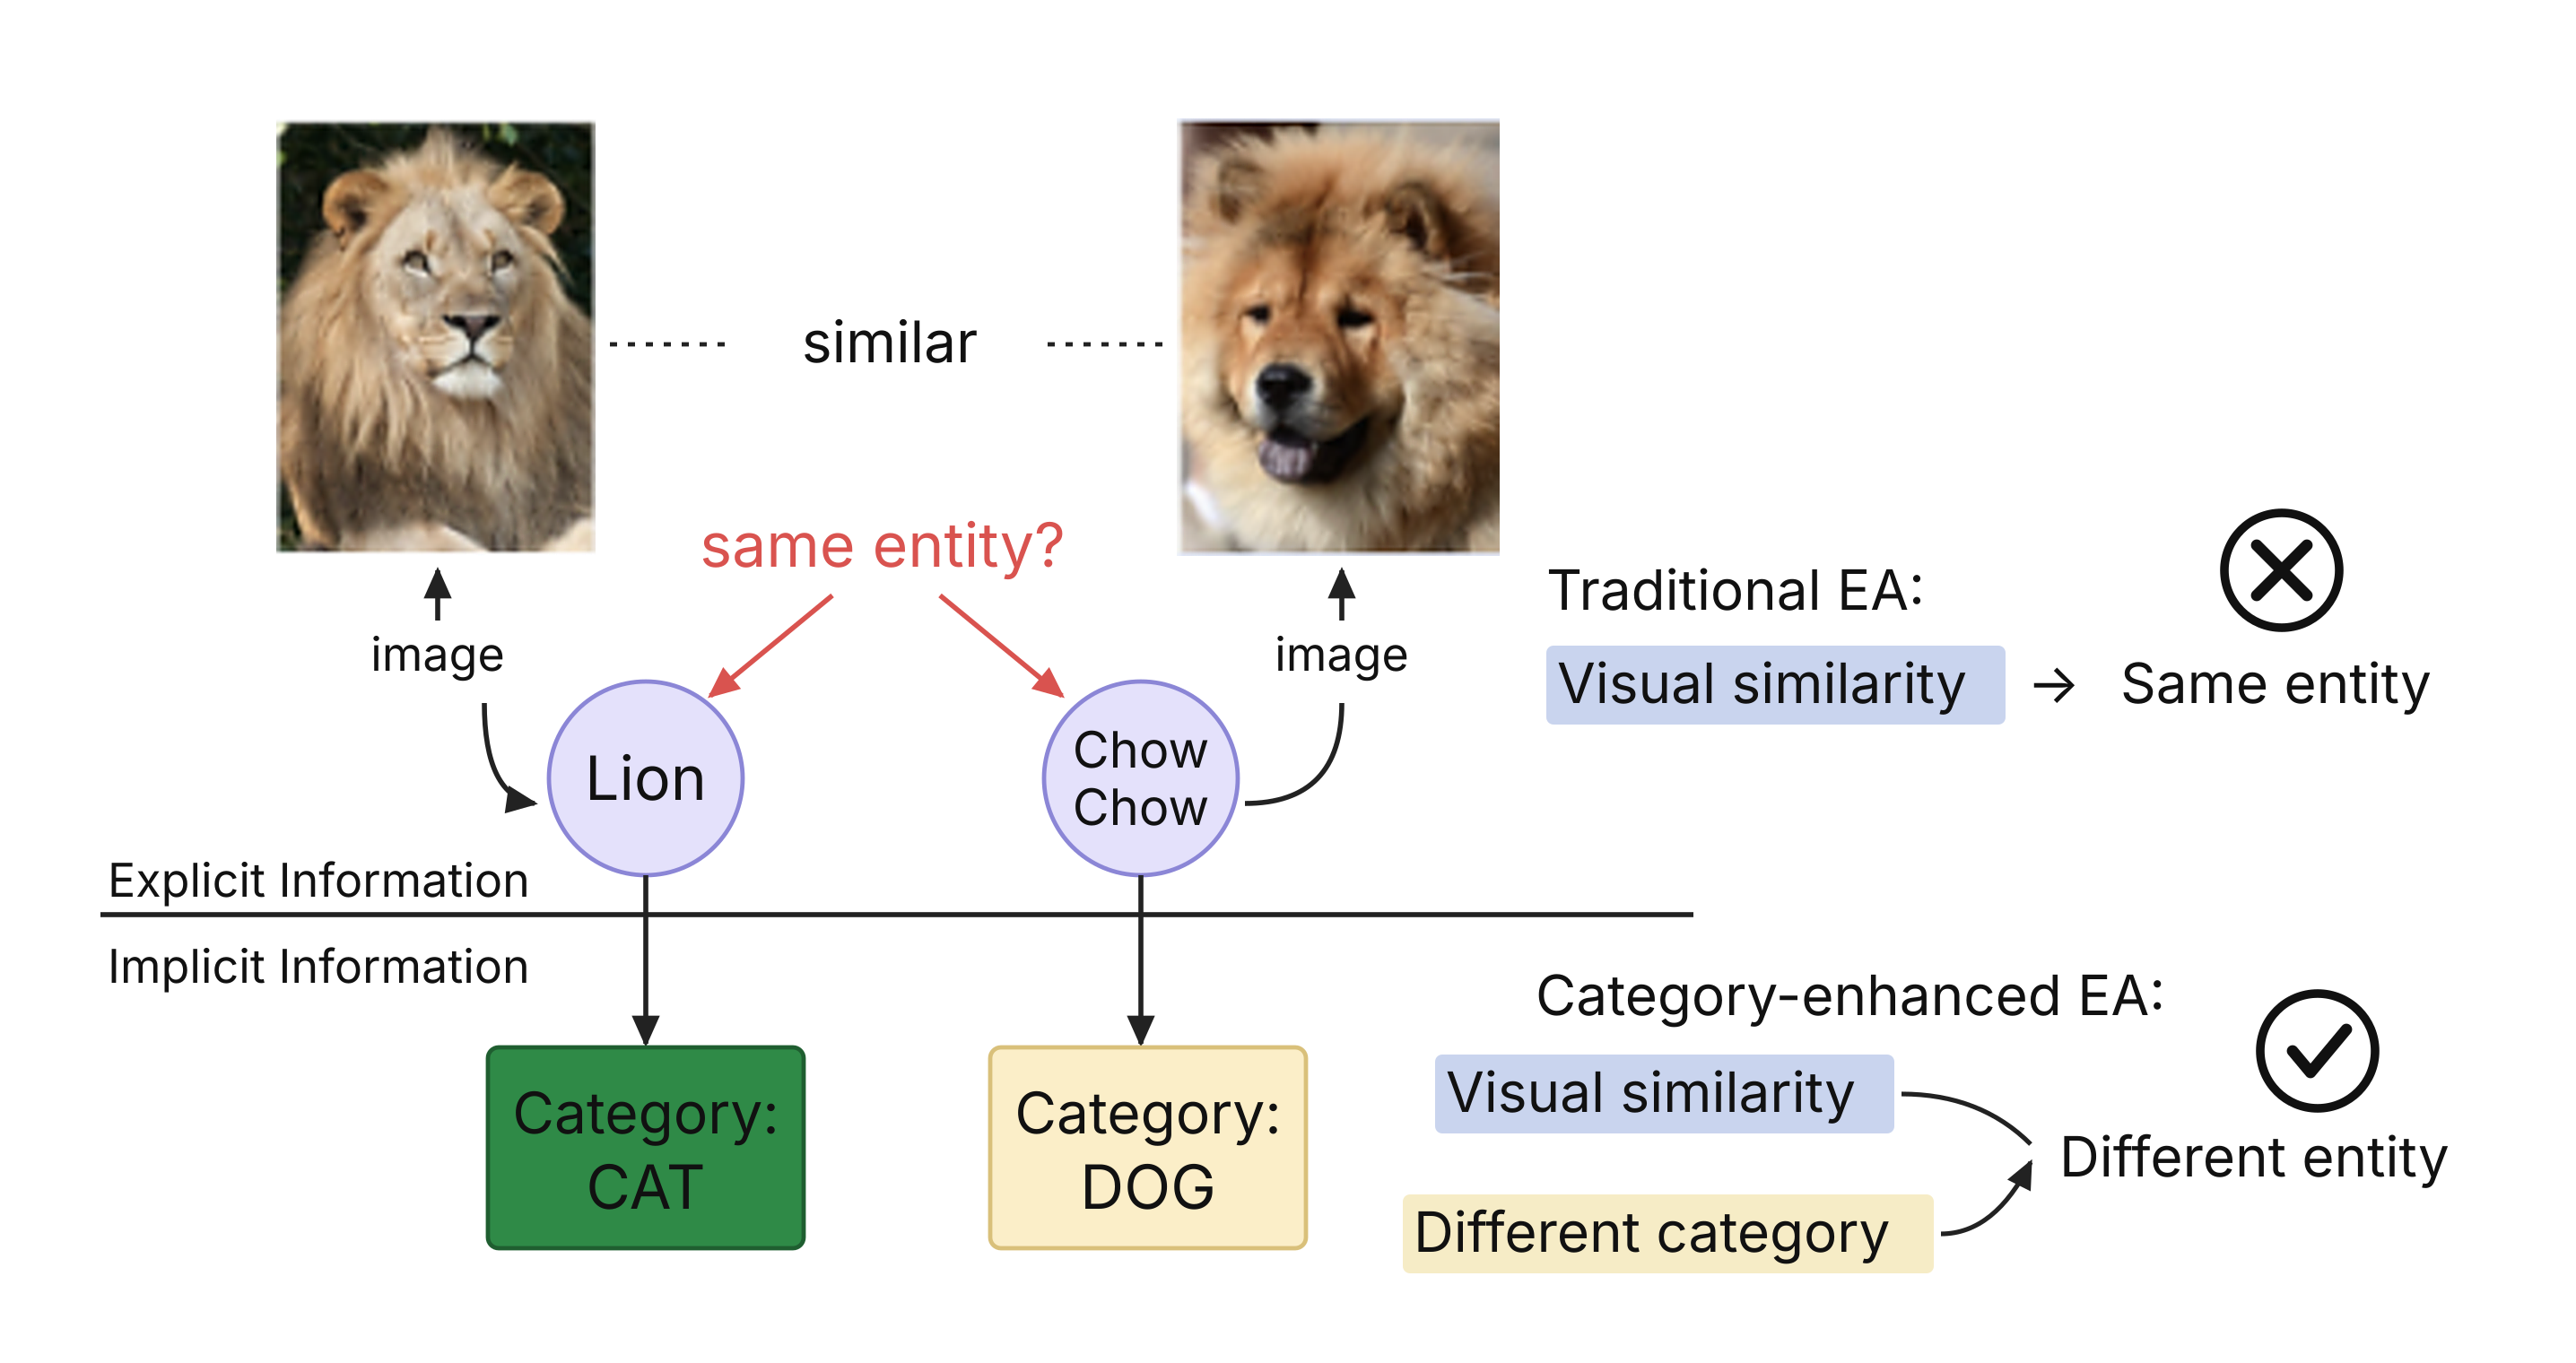
\includegraphics[width=\columnwidth]{figures/exp_1.png}
\caption{Ví dụ về việc căn chỉnh nhầm khi chỉ dựa trên độ tương đồng thị giác, và cách thông tin danh mục ngầm giúp phân biệt. Nguồn: \cite{feng-etal-2025-cateea}.}
\label{fig:cateea_idea}
\end{figure}

Để giải quyết vấn đề này, nhóm tác giả đã đề xuất phương pháp CateEA - với ý tưởng chính là đưa thông tin danh mục ngầm vào quá trình căn chỉnh thực thể để giảm những nhầm lẫn như trên.

\subsection{Phương pháp và phân tích}

CateEA gồm ba modules chính (Hình~\ref{fig:cateea_pipeline}):
\begin{itemize}
    \item \textit{Multi-Modal Encoder (MME):} Mã hoá từng nguồn thông tin rồi tổng hợp thành joint embedding.
    \item \textit{Contrastive Representation Learning (CRL):} Sử dụng phương pháp học tương phản để tinh chỉnh các embedding.
    \item \textit{Category Information Enhancement (CIE):} Khai thác thông tin danh mục ngầm để cải thiện việc căn chỉnh các thực thể.
    
\end{itemize}

\begin{figure*}[t]
\centering
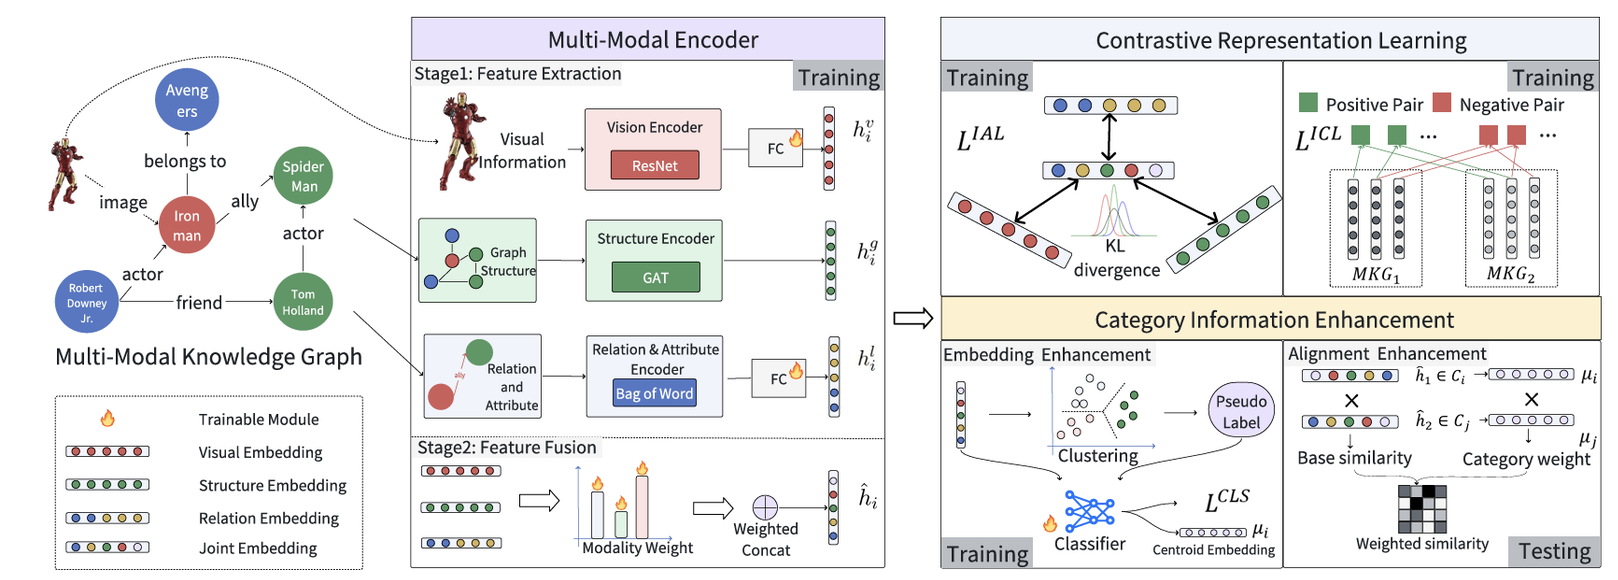
\includegraphics[width=\textwidth]{figures/pipeline.png}
\caption{Kiến trúc tổng quan của CateEA. Các modality được mã hóa rồi kết hợp thành một joint embedding duy nhất. Joint embedding này được tinh chỉnh qua module CRL để các thực thể tương ứng nằm gần nhau hơn. Song song đó, các embedding được phân cụm để tạo pseudo-category, và thông tin danh mục này được dùng để hỗ trợ huấn luyện và điều chỉnh độ tương đồng giữa các cặp thực thể. Nguồn: \cite{feng-etal-2025-cateea}, Fig. 2. Lưu ý: hình gốc chưa đánh dấu GAT là trainable; trong mã nguồn, các tham số GAT vẫn được cập nhật khi huấn luyện.}
\label{fig:cateea_pipeline}
\end{figure*}

\subsubsection{Xây dựng và học biểu diễn đa phương thức} %Hùng
% MME: mã hóa từng nguồn thông tin và kết hợp embedding.
% CRL: vai trò của ICL và IAL.
% Phân tích ý nghĩa và lựa chọn thiết kế ngay tại phần tương ứng.

Hai module MME và CRL là phần nền của CateEA, có nhiệm vụ tạo ra joint embedding của thực thể và học embedding đó cho bài toán căn chỉnh. Hai module này kế thừa nhiều từ các công trình MMEA trước đó như MCLEA\cite{lin-etal-2022-mclea}, MEAformer\cite{chen2023meaformer} nên không phải là đóng góp chính của tác giả. Nhóm chỉ trình bày ở mức cần thiết để hiểu module khai thác danh mục ngầm ở phần sau.

\paragraph{Multi-Modal Encoder (MME)}

MME dùng một bộ encoder riêng cho mỗi phương thức: 
\begin{itemize}
    \item \textit{Với cấu trúc đồ thị:}
        Sử dụng mạng GAT hai tầng để tổng hợp
        thông tin từ các thực thể lân cận thông qua
        cơ chế attention. Mỗi tầng tổng hợp thông tin
        từ các láng giềng trực tiếp, cho phép embedding
        ở tầng cuối tiếp nhận thông tin từ vùng lân cận
        tối đa hai bước (2-hop). Đầu ra là embedding
        cấu trúc $\mathbf{h}^g_i$. %Toàn sửa

    \item \textit{Với quan hệ, thuộc tính và tên}, mỗi loại $l \in \{r, a, n\}$ được biểu diễn bằng bag-of-words rồi đưa qua một lớp tuyến tính $\mathbf{h}^l_i = \mathbf{W}_l \mathbf{u}^l_i + \mathbf{b}_l$. Riêng với tên, vector đầu vào là trung bình các vector GloVe đã huấn luyện sẵn của các từ trong tên.

    \item \textit{Với hình ảnh:} Ảnh của thực thể được đưa qua ResNet-152 đã huấn luyện sẵn, lấy logits của lớp fully connected cuối cùng rồi qua một lớp tuyến tính để được $\mathbf{h}^v_i$.
\end{itemize}

Sau khi có embedding của từng modality, joint embedding được tạo bằng cách nối chúng lại, mỗi modality được nhân với một trọng số attention:
\[
    \hat{\mathbf{h}}_i
    = \bigoplus_{m \in \mathcal{M}}
    \frac{\exp(w_m)}{\sum_{j \in \mathcal{M}} \exp(w_j)}\,\mathbf{h}^m_i.
\]
Ở đây $\mathcal{M}=\{g,r,a,n,v\}$, $\oplus$ là phép nối vector và $w_m$ là trọng số attention học được của modality $m$.


\noindent\textit{Nhận xét của nhóm:} $w_m$ là tham số dùng chung cho mọi thực thể, nên mô hình chỉ học được modality nào nhìn chung đáng tin hơn, chứ không điều chỉnh riêng cho từng thực thể. Cách này đơn giản hơn MEAformer\cite{chen2023meaformer}, nơi trọng số modality thay đổi theo từng thực thể. Khi một thực thể thiếu ảnh hoặc thiếu thuộc tính thì modality đó vẫn được gán trọng số như các thực thể khác. Ngoài ra, nhóm thấy nhóm đặc trưng SF ảnh hưởng rất lớn đến kết quả. Ở cả bài báo và kết quả tái lập trên DBP15K, Hits@1 khi có SF đều trên 94\%, còn khi không có SF chỉ khoảng 74--78\% ở chế độ non-iterative. Điều này cho thấy việc bổ sung nhóm đặc trưng SF cải thiện đáng kể kết quả trên DBP15K. Trong cấu hình tái lập, w/o SF tắt cả đặc trưng tên và ký tự, nên so sánh này chưa tách riêng đóng góp của tên thực thể hay của từng phương thức.

\paragraph{Contrastive Representation Learning (CRL)}

Joint embedding từ MME chưa được đảm bảo là các thực thể tương ứng nằm gần nhau, nên CRL huấn luyện embedding theo hướng đó. Với mỗi cặp thực thể $(e^1_i, e^2_i)$ trong tập seed, các thực thể còn lại của cả hai đồ thị được xem là mẫu âm $\mathcal{N}^{neg}_i$. Xác suất căn chỉnh của modality $m$ được tính như sau:
\[
    q_m(e^1_i, e^2_i)
    = \frac{\delta_m(e^1_i, e^2_i)}
    {\delta_m(e^1_i, e^2_i)
    + \sum_{e_j \in \mathcal{N}^{neg}_i}
    \left[\delta_m(e_j, e^1_i) + \delta_m(e^2_i, e_j)\right]},
\]
với $\delta_m(u,v) = \exp\!\left(f_m(u)^\top f_m(v) / \tau_1\right)$, $f_m(\cdot)$ là encoder của modality $m$ và $\tau_1$ là nhiệt độ.

Module CRL gồm hai hàm loss:
\begin{itemize}
    \item \textit{ICL (Intra-modal Contrastive Learning):} Với từng modality, kéo cặp thực thể tương ứng lại gần nhau và đẩy các thực thể khác ra xa:
    \[
        \mathcal{L}^{ICL}_m = -\mathbb{E}_{i \in B}\log
        \tfrac{1}{2}\left[q_m(e^1_i, e^2_i) + q_m(e^2_i, e^1_i)\right].
    \]
  \item \textit{IAL (Inter-modal Alignment Learning):} Tính các vector phân phối xác suất $\mathbf{q}'_o$ từ joint embedding và $\mathbf{q}'_m$ từ modality $m$ trên cùng tập ứng viên, sử dụng nhiệt độ $\tau_2$. Sau đó, sử dụng KL divergence để đưa phân phối của modality $m$ tiệm cận với phân phối của joint embedding theo cả hai chiều:

    \begin{equation}
        \begin{aligned}
        \mathcal{L}^{IAL}_m
        = \frac{1}{2}\mathbb{E}_{i \in B}\Big[
        &\operatorname{KL}\big(
        \mathbf{q}'_o(e^1_i,\cdot)
        \,\|\, \mathbf{q}'_m(e^1_i,\cdot)
        \big)\\
        +&\operatorname{KL}\big(
        \mathbf{q}'_o(e^2_i,\cdot)
        \,\|\, \mathbf{q}'_m(e^2_i,\cdot)
        \big)
        \Big].
        \end{aligned}
    \end{equation}
    Ở đây $\mathbf{q}'_m(u,\cdot)$ là vector xác suất của các
    ứng viên khi truy vấn là $u$; mỗi phần tử tương ứng với một
    ứng viên. KL được tính trên toàn bộ hai vector phân phối,
    không chỉ trên xác suất của riêng cặp thực thể tương ứng.

\end{itemize}

Nhóm hiểu hai hàm loss này bổ sung cho nhau. ICL chỉ xét từng modality riêng lẻ nên các modality có thể học theo những hướng khác nhau, còn IAL buộc từng modality phải nhất quán với joint embedding. Nhờ vậy một modality yếu hoặc nhiễu (chẳng hạn ảnh không rõ) vẫn nhận được tín hiệu từ các modality mạnh hơn.

\subsubsection{Khai thác thông tin danh mục ngầm}
% CEE: phân cụm, tạo nhãn giả và học phân loại.
% CAE: tính trọng số danh mục và điều chỉnh điểm căn chỉnh.
% Phân biệt huấn luyện với suy luận; phân tích các giả định.

Đây là module mang tính novelty và là đóng góp chính của CateEA.

Module này có hai thành phần là \textit{Category Embedding Enhancement} và \textit{Category Alignment Enhancement}:

\paragraph{Category Embedding Enhancement (CEE)}


Đầu tiên, mô hình đã có joint embedding của thực thể, được tạo bởi module MME và được tối ưu thông qua CRL. Nhiệm vụ của CEE là phân cụm những embedding này bằng K-Medoids và lấy kết quả phân cụm làm nhãn danh mục giả (pseudo-category label). Sau đó, classifier học dự đoán nhãn giả từ embedding. Loss phân loại cross-entropy được kết hợp với loss căn chỉnh và truyền ngược về encoder để điều chỉnh biểu diễn. Tác giả nói rằng cơ chế này tương tự ý tưởng trong công trình DeepCluster năm 2018 \cite{caron2018deepcluster}.

Loss phân loại không trực tiếp kéo các embedding cùng cụm lại gần nhau, mà khuyến khích encoder tạo ra các embedding có những đặc điểm giúp phân biệt các danh mục với nhau. Luồng gradient từ loss phân loại về encoder được xác nhận trong code; tuy nhiên, việc ghép nhãn giả với embedding có sai khác sẽ được phân tích ở phần đối chiếu mã nguồn.

Việc phân cụm này không tự tạo thêm dữ liệu hay tri thức từ bên ngoài. Nó tổ chức lại những đặc điểm đã có trong không gian embedding, rồi biến cách tổ chức đó thành tín hiệu giám sát bổ sung. Ngoài ra "danh mục ngầm - implicit category" chưa chắc đã tương ứng với các danh mục thực sự ngoài thế giới thật. Phương pháp của tác giả đề xuất cơ chế này dựa trên ý tưởng khai thác thông tin danh mục ngầm ngoài thế giới thực, nhưng tác giả chưa chỉ ra các embedding trong cùng một cụm có thuộc một danh mục nào đó ngoài thực tế hay không.


Ngoài loss của classifier, nhóm còn quan tâm đến cấu trúc phân cụm. Paper sử dụng K-Medoids để chia các embedding thành $k$ cụm ở một cấp, với $k$ được xác định trước, không xây dựng các cụm cha-con hay phân cụm lồng nhau. Tác giả giải thích việc chọn K-Medoids dựa trên đặc điểm sử dụng điểm dữ liệu thực làm đại diện cụm và khả năng chống chịu nhiễu, outlier,... Tuy nhiên, paper chưa cung cấp thực nghiệm so sánh với các phương pháp phân cụm khác để kiểm chứng lợi ích của lựa chọn này trong CateEA. Phần phân tích tham số của tác giả chỉ khảo sát ảnh hưởng của số cụm $k$ khi sử dụng K-Medoids \cite{feng-etal-2025-cateea}. Và lưu ý rằng việc phân cụm chỉ xảy ra ở quá trình training. Ở quá trình inference, encoder MME đã được huấn luyện với các mục tiêu CRL tạo ra embedding để classifier dự đoán nhãn danh mục ngầm, không chạy lại CRL hay thuật toán clustering.

\paragraph{Category Alignment Enhancement (CAE)}

Thành phần CEE đã tác động vào embedding trong quá trình training, còn CAE tiếp tục sử dụng thông tin danh mục để điều chỉnh xếp hạng ứng viên. Trong mã nguồn, ở giai đoạn suy luận, classifier dự đoán nhãn danh mục giả $c_x$, $c_y$ cho hai thực thể $x$, $y$ tương ứng từ joint embedding mà không chạy lại K-Medoids. Các thực thể cùng nhãn trong mỗi đồ thị được gom nhóm thành $C_i$. Bốn bước CAE được mô tả ở paper:

\begin{itemize}
    \item Tính centroid của mỗi danh mục bằng trung bình joint embedding của các thực thể thuộc danh mục đó.
    \[
        \boldsymbol{\mu}_i
        = \frac{1}{|C_i|}
        \sum_{x \in C_i} \hat{\mathbf{h}}_x.
    \]
    \item Đo khoảng cách giữa hai danh mục, rồi chuyển thành độ tương đồng. Centroid càng gần nhau thì $s_{ij}$ càng lớn.

    \[
        d_{ij} = \|\boldsymbol{\mu}_i - \boldsymbol{\mu}_j\|_2,
        \qquad
        s_{ij} = \frac{1}{1 + d_{ij}}.
    \]
    \item Chuẩn hóa trọng số bằng softmax:

    \[
        w_{ij}
        = \frac{\exp(s_{ij})}
        {\sum_{k=1}^{C} \exp(s_{ik})}.
    \]
    \item Điều chỉnh độ tương đồng thực thể:
    \[
        S'(x,y)
        = w_{c_x,c_y}\,S(x,y).
    \]
\end{itemize}

Ký hiệu $\hat{\mathbf{h}}_x$ là joint embedding của $x$; $\boldsymbol{\mu}_i$ là centroid của $C_i$; $C$ là số danh mục. $d_{ij},s_{ij},w_{ij}$ lần lượt là khoảng cách, độ tương đồng và trọng số giữa hai danh mục. $S,S'$ là độ tương đồng thực thể trước và sau điều chỉnh.

\noindent\textit{Một nhận xét của nhóm:} Paper chọn K-Medoids vì paper lý giải rằng medoid là điểm dữ liệu thực, giúp tâm cụm mang tính đại diện và ít ảnh hưởng bởi nhiễu; nhưng ở giai đoạn suy luận lại dùng centroid (vector trung bình) không nhất thiết trùng với embedding của bất kì thực thể nào để tính khoảng cách giữa các danh mục. Paper không phân tích rõ lý do lựa chọn centroid ở bước này.

Nhóm cũng cho rằng CAE đang dựa trên giả thuyết: khoảng cách giữa các centroid thể hiện mức độ phù hợp giữa các danh mục cho việc căn chỉnh. Vấn đề nhóm thấy là centroid là biểu diễn giá trị trung bình, chưa phản ánh độ phân tán thực thể bên trong nhóm đó. Ngoài ra nếu classifier dự đoán sai nhãn, sai số này có thể ảnh hưởng đến cả centroid và trọng số hiệu chỉnh. Vì vậy, CAE không đảm bảo luôn cải thiện xếp hạng. 

Hình~\ref{alg:cateea} tóm tắt luồng khai thác danh mục ngầm
được nhóm diễn giải lại theo mô tả phương pháp trong bài báo.
Giả mã tách hai giai đoạn huấn luyện và suy luận; các sai khác
của mã nguồn công khai được phân tích tại
mục~\ref{sec:cateea_code_comparison}.

\begin{figure}[t]
\footnotesize
\begin{algorithmic}[1]
\REQUIRE Graphs $G_1,G_2$ with entity sets $E_1,E_2$;
    training alignment pairs $\mathcal{A}$; number of clusters $C$.
\ENSURE Ranked candidates for each query entity.
\STATE Initialize encoder $f_\theta$ and classifier $g_\phi$.
\STATE \textbf{Training: clustering and pseudo-label learning}
\REPEAT
    \STATE Compute $\hat{\mathbf{h}}_e=f_\theta(e)$ for
        $e\in E_1\cup E_2$.
    \STATE Cluster all embeddings with K-Medoids;
        use cluster indices as pseudo-labels $y_e$.
    \FOR{each batch of alignment pairs from $\mathcal{A}$}
        \STATE Recompute embeddings for entities in the batch.
        \STATE Predict category distributions
            $\mathbf{p}_e=g_\phi(\hat{\mathbf{h}}_e)$.
        \STATE Compute $\mathcal{L}_{\mathrm{cls}}$
            as cross-entropy between $\mathbf{p}_e$ and $y_e$.
        \STATE $\mathcal{L}=\mathcal{L}_{\mathrm{align}}
            +\lambda\mathcal{L}_{\mathrm{cls}}$.
        \STATE Backpropagate to update $\theta,\phi$;
            keep pseudo-labels fixed during this update.
    \ENDFOR
\UNTIL{the training stopping criterion is met}
\STATE \textbf{Inference: classification and ranking adjustment}
\STATE Recompute embeddings using the trained encoder.
\FOR{$g\in\{1,2\}$}
    \STATE Predict $c_e=\arg\max_c g_\phi(
        \hat{\mathbf{h}}_e)_c$ for each $e\in E_g$.
    \STATE Form groups $C_a^{(g)}=\{e\in E_g:c_e=a\}$;
        compute each centroid $\boldsymbol{\mu}_a^{(g)}$
        as the mean embedding of its group.
\ENDFOR
\STATE For each cross-graph category pair, compute
    $d_{ab}=\|\boldsymbol{\mu}_a^{(1)}
    -\boldsymbol{\mu}_b^{(2)}\|_2$ and $s_{ab}=1/(1+d_{ab})$.
\STATE Normalize $w_{ab}=\exp(s_{ab})/\sum_k\exp(s_{ak})$.
\FOR{each query entity $x\in E_1$}
    \STATE For each candidate $y\in E_2$, compute
        $S'(x,y)=w_{c_x,c_y}S(x,y)$.
    \STATE Rank candidates by decreasing $S'(x,y)$;
        apply the same procedure in the reverse direction.
\ENDFOR
\end{algorithmic}
\caption{Luồng khai thác danh mục ngầm do nhóm diễn giải lại
    theo mô tả CateEA~\cite{feng-etal-2025-cateea}.
    Lược đồ huấn luyện minh họa việc tạo nhãn giả rồi học với
    các nhãn đó, không đặc tả lịch cập nhật của mã nguồn.
    K-Medoids chỉ dùng trong huấn luyện; suy luận dùng classifier.
    Các centroid được tính cho những nhóm không rỗng.}
\label{alg:cateea}
\end{figure}
\subsection{Tái lập thực nghiệm}

% Declare wide result tables early to keep them within the CateEA section.
\begin{table*}[!t]
\centering
\caption{So sánh Hits@1, Hits@10 và MRR (\%) trên DBP15K; đối chiếu Tables 1--2 của bài báo.}
\label{tab:cateea_dbp15k}
\small
\renewcommand{\arraystretch}{1.12}
\setlength{\tabcolsep}{4pt}
\begin{tabular}{@{}llrrr@{\hspace{10pt}}rrr@{\hspace{10pt}}rrr@{}}
\toprule
\textbf{Cấu hình} & \textbf{Kết quả} & \multicolumn{3}{c}{\textbf{ZH-EN}} & \multicolumn{3}{c}{\textbf{JA-EN}} & \multicolumn{3}{c}{\textbf{FR-EN}} \\
\cmidrule(lr){3-5}\cmidrule(lr){6-8}\cmidrule(lr){9-11}
 &  & \textbf{H@1$\uparrow$} & \textbf{H@10$\uparrow$} & \textbf{MRR$\uparrow$} & \textbf{H@1$\uparrow$} & \textbf{H@10$\uparrow$} & \textbf{MRR$\uparrow$} & \textbf{H@1$\uparrow$} & \textbf{H@10$\uparrow$} & \textbf{MRR$\uparrow$} \\
\midrule
Non-iter w/o SF & Paper & 77.60 & 95.50 & 83.90 & 77.20 & 96.30 & 84.00 & 78.60 & 97.20 & 85.50 \\
 & Tái lập & \cateearun{smwb7h2s}{73.75} & \cateearun{smwb7h2s}{94.82} & \cateearun{smwb7h2s}{81.27} & \cateearun{1i8acfog}{76.02} & \cateearun{1i8acfog}{96.19} & \cateearun{1i8acfog}{83.34} & \cateearun{cs880n51}{78.14} & \cateearun{cs880n51}{97.25} & \cateearun{cs880n51}{85.22} \\
 & $\Delta$ & \deltaneg{-3.85} & \deltaneg{-0.68} & \deltaneg{-2.63} & \deltaneg{-1.18} & \deltaneg{-0.11} & \deltaneg{-0.66} & \deltaneg{-0.46} & \deltapos{+0.05} & \deltaneg{-0.28} \\
\addlinespace[3pt]
Non-iter w/ SF & Paper & 94.50 & 99.30 & 96.40 & 97.20 & 99.80 & 98.70 & 99.10 & 100.00 & 99.50 \\
 & Tái lập & \cateearun{ouxqphvg}{94.20} & \cateearun{ouxqphvg}{99.27} & \cateearun{ouxqphvg}{96.13} & \cateearun{i448247f}{97.13} & \cateearun{i448247f}{99.85} & \cateearun{i448247f}{98.25} & \cateearun{h9llx682}{99.01} & \cateearun{h9llx682}{99.98} & \cateearun{h9llx682}{99.43} \\
 & $\Delta$ & \deltaneg{-0.30} & \deltaneg{-0.03} & \deltaneg{-0.27} & \deltaneg{-0.07} & \deltapos{+0.05} & \deltaneg{-0.45} & \deltaneg{-0.09} & \deltaneg{-0.02} & \deltaneg{-0.07} \\
\addlinespace[3pt]
Iter w/o SF & Paper & 83.90 & 97.10 & 88.70 & 85.10 & 97.80 & 89.90 & 86.20 & 98.50 & 90.80 \\
 & Tái lập & \cateearun{yhxmaaiy}{79.58} & \cateearun{yhxmaaiy}{95.69} & \cateearun{yhxmaaiy}{85.48} & \cateearun{anh3017u}{82.68} & \cateearun{anh3017u}{97.07} & \cateearun{anh3017u}{88.11} & \cateearun{yfsixay2}{84.77} & \cateearun{yfsixay2}{98.00} & \cateearun{yfsixay2}{89.78} \\
 & $\Delta$ & \deltaneg{-4.32} & \deltaneg{-1.41} & \deltaneg{-3.22} & \deltaneg{-2.42} & \deltaneg{-0.73} & \deltaneg{-1.79} & \deltaneg{-1.43} & \deltaneg{-0.50} & \deltaneg{-1.02} \\
\addlinespace[3pt]
Iter w/ SF & Paper & 97.40 & 99.80 & 98.40 & 99.20 & 99.90 & 99.30 & 99.70 & 100.00 & 99.80 \\
 & Tái lập & \cateearun{vzdpd3hi}{97.24} & \cateearun{vzdpd3hi}{99.71} & \cateearun{vzdpd3hi}{98.22} & \cateearun{0sp0eyep}{98.84} & \cateearun{0sp0eyep}{99.97} & \cateearun{0sp0eyep}{99.31} & \cateearun{xvueasz7}{99.64} & \cateearun{xvueasz7}{100.00} & \cateearun{xvueasz7}{99.81} \\
 & $\Delta$ & \deltaneg{-0.16} & \deltaneg{-0.09} & \deltaneg{-0.18} & \deltaneg{-0.36} & \deltapos{+0.07} & \deltapos{+0.01} & \deltaneg{-0.06} & 0.00 & \deltapos{+0.01} \\
\bottomrule
\end{tabular}
\vspace{3pt}
\begin{tablenotes}[flushleft]
\footnotesize
\item \textit{Nhấn vào các số liệu có nền xám
để xem kết quả thực nghiệm tương ứng trên W\&B.}
\end{tablenotes}
\end{table*}

\begin{table*}[!t]
\centering
\caption{So sánh Hits@1, Hits@10 và MRR (\%) trên MMKB; đối chiếu Tables 3--4 của bài báo.}
\label{tab:cateea_mmkb}
\small
\renewcommand{\arraystretch}{1.12}
\setlength{\tabcolsep}{6pt}
\begin{tabular}{@{}lllrrr@{\hspace{14pt}}rrr@{}}
\toprule
\textbf{Chế độ} & \textbf{Tỷ lệ} & \textbf{Kết quả} & \multicolumn{3}{c}{\textbf{FB15K-DB15K}} & \multicolumn{3}{c}{\textbf{FB15K-YAGO15K}} \\
\cmidrule(lr){4-6}\cmidrule(lr){7-9}
 &  &  & \textbf{H@1$\uparrow$} & \textbf{H@10$\uparrow$} & \textbf{MRR$\uparrow$} & \textbf{H@1$\uparrow$} & \textbf{H@10$\uparrow$} & \textbf{MRR$\uparrow$} \\
\midrule
Non-iter & 20\% & Paper & 49.30 & 75.90 & 58.40 & 40.20 & 67.50 & 49.70 \\
 &  & Tái lập & \cateearun{dccl235x}{48.88} & \cateearun{dccl235x}{75.65} & \cateearun{dccl235x}{58.18} & \cateearun{u7l7rzah}{38.84} & \cateearun{u7l7rzah}{66.26} & \cateearun{u7l7rzah}{48.22} \\
 &  & $\Delta$ & \deltaneg{-0.42} & \deltaneg{-0.25} & \deltaneg{-0.22} & \deltaneg{-1.36} & \deltaneg{-1.24} & \deltaneg{-1.48} \\
\addlinespace[3pt]
Non-iter & 50\% & Paper & 67.40 & 87.40 & 74.50 & 60.80 & 82.90 & 68.60 \\
 &  & Tái lập & \cateearun{vckjpp3o}{66.01} & \cateearun{vckjpp3o}{86.16} & \cateearun{vckjpp3o}{73.20} & \cateearun{9060trns}{60.19} & \cateearun{9060trns}{81.83} & \cateearun{9060trns}{67.84} \\
 &  & $\Delta$ & \deltaneg{-1.39} & \deltaneg{-1.24} & \deltaneg{-1.30} & \deltaneg{-0.61} & \deltaneg{-1.07} & \deltaneg{-0.76} \\
\addlinespace[3pt]
Non-iter & 80\% & Paper & 79.90 & 93.30 & 84.90 & 74.20 & 91.20 & 80.50 \\
 &  & Tái lập & \cateearun{92xpyrkt}{77.16} & \cateearun{92xpyrkt}{91.61} & \cateearun{92xpyrkt}{82.52} & \cateearun{iovu8zta}{74.22} & \cateearun{iovu8zta}{90.82} & \cateearun{iovu8zta}{80.36} \\
 &  & $\Delta$ & \deltaneg{-2.74} & \deltaneg{-1.69} & \deltaneg{-2.38} & \deltapos{+0.02} & \deltaneg{-0.38} & \deltaneg{-0.14} \\
\addlinespace[3pt]
Iter & 20\% & Paper & 59.90 & 82.20 & 67.50 & 51.80 & 74.50 & 59.40 \\
 &  & Tái lập & \cateearun{gustc0d9}{62.31} & \cateearun{gustc0d9}{82.45} & \cateearun{gustc0d9}{69.39} & \cateearun{ownvumgr}{52.17} & \cateearun{ownvumgr}{73.46} & \cateearun{ownvumgr}{59.58} \\
 &  & $\Delta$ & \deltapos{+2.41} & \deltapos{+0.25} & \deltapos{+1.89} & \deltapos{+0.37} & \deltaneg{-1.04} & \deltapos{+0.18} \\
\addlinespace[3pt]
Iter & 50\% & Paper & 70.50 & 88.20 & 76.40 & 64.00 & 84.40 & 70.80 \\
 &  & Tái lập & \cateearun{mdwrjgz5}{70.55} & \cateearun{mdwrjgz5}{86.93} & \cateearun{mdwrjgz5}{76.35} & \cateearun{wywowfuy}{64.43} & \cateearun{wywowfuy}{82.53} & \cateearun{wywowfuy}{70.81} \\
 &  & $\Delta$ & \deltapos{+0.05} & \deltaneg{-1.27} & \deltaneg{-0.05} & \deltapos{+0.43} & \deltaneg{-1.87} & \deltapos{+0.01} \\
\addlinespace[3pt]
Iter & 80\% & Paper & 80.60 & 93.40 & 85.30 & 74.60 & 91.50 & 80.70 \\
 &  & Tái lập & \cateearun{t0eainhm}{80.18} & \cateearun{t0eainhm}{92.55} & \cateearun{t0eainhm}{84.65} & \cateearun{oxqvbkz1}{74.71} & \cateearun{oxqvbkz1}{89.33} & \cateearun{oxqvbkz1}{79.98} \\
 &  & $\Delta$ & \deltaneg{-0.42} & \deltaneg{-0.85} & \deltaneg{-0.65} & \deltapos{+0.11} & \deltaneg{-2.17} & \deltaneg{-0.72} \\
\bottomrule
\end{tabular}
\end{table*}


\subsubsection{Thiết lập thực nghiệm}

Nhóm sử dụng mã nguồn công khai của tác giả và bổ sung các script chạy, ghi nhận kết quả bằng Weights \& Biases (W\&B), cùng chức năng lưu checkpoint. Mã nguồn và hướng dẫn chạy lại được cung cấp tại \href{https://github.com/keiranoluv/Reproduce_CateEA}{GitHub}.

Theo cấu hình được ghi nhận trong repository, môi trường thực nghiệm sử dụng Ubuntu 24.04, GPU NVIDIA GeForce RTX 5090 với 32 GB VRAM, Python 3.12 và PyTorch 2.13.0 với CUDA 13.0. Dữ liệu được lấy từ gói dữ liệu do MEAformer cung cấp, gồm:
\begin{itemize}
    \item \textit{DBP15K:} ba cặp ngôn ngữ ZH-EN, JA-EN và FR-EN, với tỷ lệ cặp thực thể huấn luyện là 30\%.
    \item \textit{MMKB:} FB15K-DB15K và FB15K-YAGO15K, với các tỷ lệ huấn luyện 20\%, 50\% và 80\%.
\end{itemize}

Trên DBP15K, nhóm chạy hai chế độ non-iterative và iterative, mỗi chế độ có cấu hình sử dụng và không sử dụng surface form (SF). Trong mã nguồn, cấu hình w/o SF tắt cả đặc trưng tên và ký tự. Trên MMKB, nhóm chạy hai chế độ với ba tỷ lệ huấn luyện, không sử dụng các đặc trưng này. Tổng cộng có 24 cấu hình thực nghiệm.

Các script đặt số epoch là 1000, learning rate $5\times10^{-4}$, batch size 512, random seed 42, $\tau_1=0.1$, $\tau_2=0.4$ và CSLS với $k=3$. Mô hình được đánh giá sau mỗi 50 epoch. Với chế độ iterative, quá trình bổ sung cặp thực thể được bật từ epoch có chỉ số 500. Chi tiết từng cấu hình được lưu trong các script của repository.

Mã nguồn ghi nhận Hits@1, Hits@10, Hits@50 và MRR theo hai chiều căn chỉnh. Checkpoint tốt nhất được chọn theo Hits@1 trung bình hai chiều của nhánh đánh giá thông thường (\texttt{test}). Nhánh có điều chỉnh danh mục (\texttt{weighted}) được đánh giá và ghi nhận riêng tại cùng checkpoint. Nhóm sử dụng kết quả của nhánh \texttt{weighted} tại checkpoint này để so sánh với bài báo.


\noindent\textit{Giới hạn của giao thức đánh giá:} Nhóm \textbf{chọn checkpoint dựa trên Hits@1 của tập kiểm tra}, thay vì một tập validation độc lập. Vì vậy, tập kiểm tra đồng thời tham gia lựa chọn mô hình và đánh giá kết quả cuối cùng, có thể khiến kết quả được báo cáo lạc quan hơn so với đánh giá trên dữ liệu chưa tham gia lựa chọn. Các kết quả CateEA cần được diễn giải cùng giới hạn này.


Các lần chạy được theo dõi tại \href{https://forge.coreweave.com/wandb/keiranoluv-hcmus/cateea-reproduction}{W\&B}.
% Bổ sung link run/report tương ứng ngay tại từng bảng kết quả.


\subsubsection{Kết quả và phân tích}

Bảng~\ref{tab:cateea_dbp15k} và Bảng~\ref{tab:cateea_mmkb}
so sánh Hits@1, Hits@10 và MRR (\%) giữa bài báo và kết quả tái lập.
$\Delta$ là chênh lệch giữa kết quả tái lập và bài báo,
tính theo \%. Bấm vào số liệu tái lập sẽ dẫn
đến run W\&B tương ứng.





Trên DBP15K (Bảng~\ref{tab:cateea_dbp15k}), Hits@1 tái lập
thấp hơn bài báo ở toàn bộ cấu hình. Khi sử dụng SF,
chênh lệch nhỏ hơn 0.4\%. Khi không sử dụng SF,
chênh lệch rõ hơn, lớn nhất là 4.32\% ở
ZH-EN iterative. Nhóm tái hiện được xu hướng các cấu hình
có SF đạt kết quả cao hơn và iterative cải thiện so với
non-iterative ở các thiết lập tương ứng. Tuy nhiên, các
kết quả này chưa đủ xác định nguyên nhân của chênh lệch
với bài báo.





Trên MMKB (Bảng~\ref{tab:cateea_mmkb}), Hits@1 tái lập
non-iterative thấp hơn bài báo ở phần lớn cấu hình.
Với iterative, năm trong sáu cấu hình đạt kết quả cao hơn
bài báo trong lần chạy này, đáng chú ý nhất là
FB15K-DB15K với tỷ lệ 20\%, cao hơn 2.41\%.

Ở các cấu hình MMKB iterative, Hits@10 chỉ cao hơn bài báo
trong một cấu hình, còn MRR cao hơn trong ba cấu hình.
Xu hướng chênh lệch với bài báo không đồng nhất giữa các metric.

Trong các kết quả tái lập, iterative đều cải thiện so với
non-iterative ở cùng bộ dữ liệu và tỷ lệ huấn luyện.
Kết quả cũng tăng khi tỷ lệ cặp huấn luyện tăng.
Tuy nhiên, vì mỗi cấu hình sử dụng một random seed,
nhóm chưa đánh giá được độ biến thiên giữa các lần chạy;
những chênh lệch nhỏ chưa đủ chứng minh sự cải thiện ổn định.

\subsection{Đánh giá và thảo luận}

\subsubsection{Đối chiếu bài báo với mã nguồn}
\label{sec:cateea_code_comparison}

Trong quá trình tìm hiểu và tái lập, nhóm ghi nhận một số sai khác giữa mô tả phương pháp và mã nguồn công khai. 

% \begin{itemize}
%     \item 
%     Paper viết việc phân cụm dựa trên joint embedding của một thực thể. Trong code, với mỗi cặp thực thể tương ứng đã biết, hai embedding này được cộng lại thành một vector mới rồi được đưa vào phân cụm.

%     \item 
%     Sau khi tạo nhãn giả cho từng cặp thực thể ở bước trên, code ghép các nhãn này với thực thể theo thứ tự trong danh sách ban đầu, thay vì gán nhãn cho đúng hai thực thể thuộc cặp tương ứng.
%     \item 
%     Paper nói rằng số cụm $C=10$ nhưng tác giả lại hardcode là $C=5$.

%     \item 
%     Paper đưa các độ tương đồng danh mục qua softmax để chuẩn hoá còn code lại thực hiện phép chia một phần tử cho tổng.

%     \item 
%     Trong paper, "trọng số danh mục" được nhân với "độ tương đồng thực thể", điểm càng lớn thì ứng viên càng được ưu tiên. Tuy nhiên, code lại nhân "trọng số danh mục" với "khoảng cách thực thể". "Trọng số danh mục" là đại lượng càng lớn càng tốt, "khoảng cách thực thể" là một đại lượng càng nhỏ càng tốt nếu ta muốn xét đến độ tương đồng, vậy mà code lại nhân hai đại lượng này với nhau.
% \end{itemize}

Nhóm đối chiếu mã nguồn CateEA tại commit
\texttt{8c277f3} với mô tả phương pháp trong bài báo và ghi nhận:
\begin{itemize}
  \item \textit{Đầu vào phân cụm:} mã nguồn tạo một vector cho
  mỗi cặp căn chỉnh $(u_i,v_i)$ bằng phép cộng
  $\hat{h}_{u_i}+\hat{h}_{v_i}$, rồi phân cụm các vector này,
  thay vì trực tiếp phân cụm từng biểu diễn thực thể.
  \footnote{\href{https://github.com/Melkor0007/CateEA/blob/8c277f3292b98f22aaaecb75d01ac44487cefed6/src/myrun.py\#L461-L474}{CateEA: tạo đầu vào và nhãn phân cụm.}}

  \item \textit{Ghép nhãn giả:} nhãn được tạo theo thứ tự các
  cặp trong \texttt{train\_ill}, nhưng loss phân loại sử dụng
  \texttt{joint\_emb[si:end\_idx]} cùng
  \texttt{cluster\_labels[si:end\_idx]}, không truy xuất
  embedding theo ID của hai thực thể trong cặp tương ứng.
  \footnote{\href{https://github.com/Melkor0007/CateEA/blob/8c277f3292b98f22aaaecb75d01ac44487cefed6/src/myrun.py\#L518-L533}{CateEA: ghép embedding và nhãn cho loss phân loại.}}
  Ví dụ minh họa với chỉ số bắt đầu từ 0: nếu hai cặp đầu là
  $(2,7)$ và $(5,9)$, nhãn $c_0,c_1$ được tạo từ
  $\hat{h}_2+\hat{h}_7$ và $\hat{h}_5+\hat{h}_9$.
  Tuy nhiên, khi xét hai dòng đầu của batch phân loại, code
  ghép $\hat{h}_0$ với $c_0$ và $\hat{h}_1$ với $c_1$.
  Cách truy xuất này không bảo toàn ánh xạ từ cặp thực thể
  sang nhãn giả. Ví dụ chỉ minh họa chỉ số, không phải dữ
  liệu quan sát từ một lần chạy cụ thể.

  \item \textit{Số cụm:} mã nguồn gán trực tiếp
  \texttt{num\_category = 5}, trong khi mục~4.1.3 của bài báo
  công bố sử dụng 10 danh mục.
  \footnote{\href{https://github.com/Melkor0007/CateEA/blob/8c277f3292b98f22aaaecb75d01ac44487cefed6/src/myrun.py\#L466-L474}{CateEA: số cụm cố định trong mã nguồn.}}

  \item \textit{Chuẩn hóa trọng số danh mục:} bài báo sử dụng
  softmax, còn code tính $w_{ij}=s_{ij}/\sum_k s_{ik}$.
  Hai phép chuẩn hóa này nói chung không tương đương.
  \footnote{\href{https://github.com/Melkor0007/CateEA/blob/8c277f3292b98f22aaaecb75d01ac44487cefed6/src/myrun.py\#L774-L782}{CateEA: chuẩn hóa trọng số danh mục.}}

  \item \textit{Đại lượng được hiệu chỉnh:} bài báo nhân trọng
  số danh mục với độ tương đồng, còn code nhân trọng số với
  khoảng cách thực thể. Sau đó code có thể áp dụng CSLS và
  xếp hạng theo giá trị khoảng cách tăng dần. Vì vậy, không
  thể đồng nhất trực tiếp cách hiệu chỉnh này với công thức
  nhân độ tương đồng trong bài báo.
  \footnote{\href{https://github.com/Melkor0007/CateEA/blob/8c277f3292b98f22aaaecb75d01ac44487cefed6/src/myrun.py\#L786-L810}{CateEA: hiệu chỉnh khoảng cách và xếp hạng.}}
\end{itemize}


Nhóm đã xác nhận các sai khác trên khi đọc mã nguồn, nhưng chưa có thực nghiệm kiểm tra riêng từng sai khác để xác định ảnh hưởng của chúng đến kết quả tái lập.


\subsubsection{Nhận xét của nhóm}

Theo nhóm, điểm đáng chú ý của CateEA là biến kết quả phân cụm thành tín hiệu giám sát bổ sung cho việc học biểu diễn, đồng thời sử dụng thông tin danh mục khi xếp hạng ứng viên. Phương pháp này không cần nhãn danh mục thủ công, nhưng hiệu quả phụ thuộc vào chất lượng nhãn giả và cách khai thác chúng.

Những phân tích ở phần phương pháp cho thấy cần phân biệt chất lượng căn chỉnh với chất lượng ngữ nghĩa của các cụm. Các benchmark và ablation của tác giả hỗ trợ đánh giá hiệu quả dự đoán, nhưng chưa trả lời đầy đủ các câu hỏi về cách hình thành và sử dụng danh mục đã nêu ở trên.

Ngoài ra kết quả tái lập cho thấy có xu hướng cải thiện từ SF trên DBP15K và từ iterative trên các cấu hình đã chạy. Tuy nhiên, những so sánh này chưa tách riêng đóng góp của CEE và CAE. Để kiểm chứng sâu hơn, nhóm cho rằng cần đối chiếu rõ kết quả có và không có CAE tại cùng checkpoint, thực hiện ablation cho CEE, kiểm tra và sửa lại từng sai khác mã nguồn và chạy nhiều random seed để đánh giá độ ổn định.